\chapter{Task 1}
\begin{parlist}
	\item Application domain classes are constructed from the  domain/requirements engineering in the system analysis, or inception, phase of a development project. They are mostly solution independent in a sense that are not bound to any platform to be developed with(they are not specifically Java classes for example). Do not represent any type of methods, they are ofter depicted with responsibilities. Often application domain classes don't depict any types for their attributes. See figure \ref{fig:ADC}. \\
		Unlike application domain classes, solution domain classes are indeed platform dependent and need methods that translates at least partially their responsibility. Compared to the previous type, SDC can often have arrows that imprint directions and therefore more precision when depicting associations between classes. SDC also have to specify types for their attributes. See figure \ref{fig:SDC}.
	\item In particular for our project:
% Side by side figures 
\begin{figure}
\begin{minipage}[c]{0.6\linewidth}
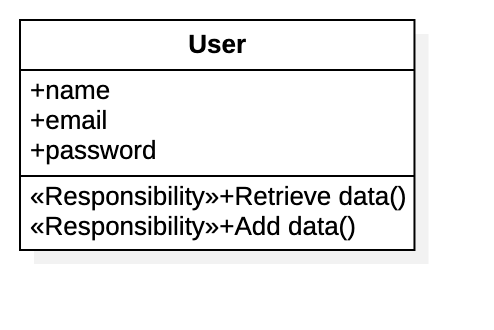
\includegraphics[width=\linewidth]{Immagini/ADC.png}
\caption{Solution Domain Class}
\label{fig:ADC}
\end{minipage}
\hfill
\begin{minipage}[c]{0.6\linewidth}
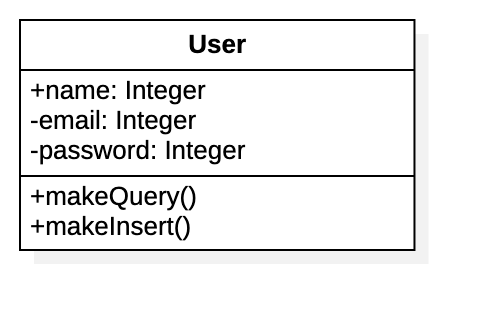
\includegraphics[width=\linewidth]{Immagini/SDC.png}
\caption{Solution Domain Class}
\label{fig:SDC}
\end{minipage}
\end{figure}	
\newpage
\item This is the table completed:
\begin{table}[hbt]
\centering
\begin{tblr}{
  cell{1}{2} = {c=3}{c},
  hlines,
  vlines,
}
                               & \textbf{Developement Phase}                  &                                                &                         \\
\textbf{Aspect}                & \textbf{Analysis}                            & \textbf{Draft}                                 & \textbf{Implementation} \\
\textit{Intended Use}          & idea focusing ~                              & idea implementing~                             & idea realizing~         \\
\textit{Terminology}           &                                              &                                                &                         \\
\textit{Class semantics}       & application domain                           & design domain                                  & solution domain         \\
\textit{Association semantics} &                                              &                                                &                         \\
\textit{Detail level}          & solution independent                         & platform independent                           & platform specific       \\
\textit{Target group}          & {stakeholders with~\\no technical knowledge} & {stakeholders with~\\some technical knowledge} & developers              
\end{tblr}
\end{table}
	

\end{parlist}